\documentclass[letterpaper, 11pt, DIV=11]{scrartcl}
\usepackage[utf8x]{inputenc}
\usepackage[T1]{fontenc}
\usepackage{../l3customlisting}
\usepackage[american]{babel}
\usepackage{mathptmx}
\usepackage{graphicx}
\usepackage{microtype}
\usepackage{metalogo}
\usepackage{caption}
\usepackage{hyperref}


\addtokomafont{disposition}{\rmfamily}
\author{\href{https://www.alanshawn.com}{Ziyue ``Alan'' Xiang}}
\title{\texttt{l3customlisting}\\Typeset Code Listings and Emulate Console Screenshots with \LaTeX\  Beautifully\\ {\small \url{https://github.com/xziyue/latex-beautiful-listings-screenshot}}}
\date{\today}


\newmintinline[texinline]{latex}{frame=none, fontsize=\fontsize{10}{10}}

\newtcblisting{tcbsrccode}[1]{
    ctmlstmintedstyle,listing engine=minted, breakable, colback=black!5, boxsep=0pt, colframe=black!30, minted options={linenos,autogobble,breaklines, numbersep=3mm, obeytabs, tabsize=2,fontsize=\fontsize{8}{8}},
    minted language=#1
}

\newenvironment{mylisting}{\medskip\captionsetup{type=listing, labelsep=colon}}{\medskip}
\DeclareCaptionType{lstcap}[Listing][List of Code Listings]

\begin{document}


\pagenumbering{Roman}

\maketitle

\tableofcontents

\clearpage

\pagenumbering{arabic}

This is the \LaTeX 3 version of the old \rawinline|customlisting| package, which allows users to control the styles and declare new listing environments more easily. The old package can be found in \href{https://github.com/xziyue/latex-beautiful-listings-screenshot/tree/master/archive}{\rawinline|archive|} folder.

\section{Quick Start Guide}

\begin{enumerate}
\item Download \href{https://github.com/xziyue/latex-beautiful-listings-screenshot/blob/master/l3customlisting.sty}{\rawinline|l3customlisting.sty|} and place it in your project folder.
\item Load the package with \texinline|\usepackage{l3customlisting}|.
\item If you are using pdf\LaTeX, make sure to include \texinline|\usepackage[T1]{fontenc}| in the preamble. Otherwise, symbols like \textasciitilde\ may not be displayed correctly.
\end{enumerate}

This package provides the following environments:
\begin{itemize}
\item \rawinline|tcbconsole|, \rawinline|tcbconsole*|
\item \rawinline|tcbcode|, \rawinline|tcbcode*|
\item \rawinline|tcbverbatim|, \rawinline|tcbverbatim*|
\end{itemize}

This package also provides the following commands:
\begin{itemize}
\item \rawinline|tcbinputcode|, \rawinline|tcbinputcode*|
\item \rawinline|tcbinputverbatim|, \rawinline|tcbinputverbatim*|
\end{itemize}

The starred environments/commands offer \emph{unbreakable} listing boxes; while normal ones are \emph{breakable}.



\section{Typeset Source Code Listings}

\begin{itemize}

\item Typeset source code inside \TeX\ files

\begin{tcbsrccode}{text}
\begin{tcbcode}{cpp}
#include <iostream>  
using namespace std; 

int main(){ 
    cout<<"Hello World\n"; 
    return 0; 
} 
\end{tcbcode}
\end{tcbsrccode}
\begin{tcbcode}{cpp}
#include <iostream>  
using namespace std; 

int main(){ 
    cout<<"Hello World\n"; 
    return 0; 
} 
\end{tcbcode}


\item Typeset source code from external source files

\begin{tcbsrccode}{text}
\tcbinputcode*{cpp}{../res/example.cpp}
\end{tcbsrccode}
\tcbinputcode*{cpp}{../res/example.cpp}

\item Inline source code

\begin{tcbsrccode}{text}
\cinline|printf("%s", "some text");|
\pyinline|map(lambda x:x, [1, 2])|
\rawinline|raw value|
\end{tcbsrccode}
\cinline|printf("%s", "some text");|
\pyinline|map(lambda x:x, [1, 2])|
\rawinline|raw value|

\item Declare inline macros for other languages

\begin{tcbsrccode}{text}
\ctmlstnewinline{rubyinline}{ruby} %{macro name}{language}
\rubyinline|puts 'Hello, world!'|
\end{tcbsrccode}
\ctmlstnewinline{rubyinline}{ruby} %{macro name}{language}
\rubyinline|puts 'Hello, world!'|

\end{itemize}

\section{Typeset Generic Verbatims}

\begin{itemize}
\item Typeset generic verbatims inside \TeX\ files

\begin{tcbsrccode}{text}
\begin{tcbverbatim}
__________________________  ___
\__    ___/\_   _____/\   \/  /
  |    |    |    __)_  \     / 
  |    |    |        \ /     \ 
  |____|   /_______  //___/\  \
                   \/       \_/
\end{tcbverbatim}
\end{tcbsrccode}
\begin{tcbverbatim}
__________________________  ___
\__    ___/\_   _____/\   \/  /
  |    |    |    __)_  \     / 
  |    |    |        \ /     \ 
  |____|   /_______  //___/\  \
                   \/       \_/
\end{tcbverbatim}


\item Typeset generic verbatims from external files

\begin{tcbsrccode}{text}
\tcbinputverbatim*{../res/wireshark.txt}
\end{tcbsrccode}
\tcbinputverbatim*{../res/wireshark.txt}

\end{itemize}


\section{Typeset Console Screenshots}

Typesetting console screenshots is a bit trickier. By far, it can be done most conveniently on Ubuntu 18.04+. The key is to convert ANSI color codes used by the console into HTML. As it is shown in Figure \ref{fig:ubuntu-conv}, on Ubuntu 18.04+, this can be done simply by selecting the desired region, right click and select ``Copy as HTML''. On other platforms, this should be also doable by dumping the terminal output to a file and using a conversion tool such as \href{https://pypi.org/project/ansi2html/}{\rawinline{ansi2html}}.

\begin{figure}[htpb]
\centering
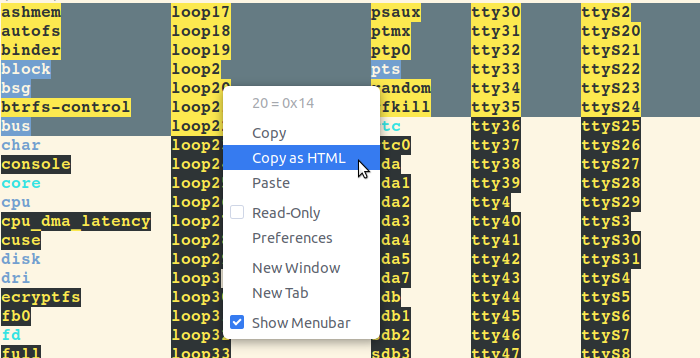
\includegraphics[width=0.6\linewidth]{../res/ubuntu-html}
\caption{Converting terminal output to HTML on Ubuntu 18.04+.}
\label{fig:ubuntu-conv}
\end{figure} 

Generally speaking, one needs to fulfill the following requirements:
\begin{enumerate}
\item Have a way of converting terminal output to HTML.
\item Be able to run the \href{https://github.com/xziyue/latex-beautiful-listings-screenshot/blob/master/html2tex_gui.py}{\rawinline|html2latex|} \LaTeX\ Python script. Currently, the script is dependent on \href{https://pypi.org/project/wxPython/}{\rawinline|wxPython|}, \href{https://pypi.org/project/TexSoup/}{\rawinline|TexSoup|} and \href{https://pypi.org/project/colour/}{\rawinline|colour|}. Please note that this software is very primitive and does not support many HTML features. If any problem occurs, you can try the old version in the \rawinline|archive| folder.
\end{enumerate}

To typeset this screenshot in \LaTeX, one needs to run \rawinline|html2latex| and paste the HTML in the upper text box. By pressing the ``Convert`` button, the corresponding \LaTeX\ code will appear in the lower text box, as it is shown in Figure \ref{fig:python-html2latex}. The result is shown as below.

\begin{tcbsrccode}{text}
\input{../res/console-dev.txt}
\end{tcbsrccode}
\input{../res/console-dev.txt}

\begin{figure}[htpb]
\centering
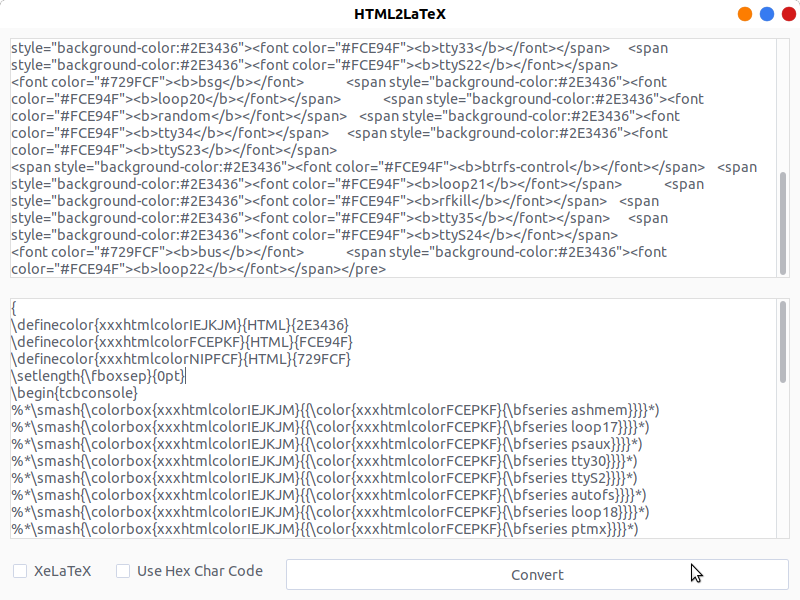
\includegraphics[width=0.7\linewidth]{../res/html2latex}
\caption{Using \rawinline|html2latex| to convert HTML to \LaTeX.}
\label{fig:python-html2latex}
\end{figure} 

Other classic command-line tools, such as \rawinline|emacs| and \rawinline|htop|, are supported as well.

\begin{tcbsrccode}{text}
\input{../res/console-emacs.txt}
\end{tcbsrccode}
\input{../res/console-emacs.txt}


\begin{tcbsrccode}{text}
\input{../res/console-htop.txt}
\end{tcbsrccode}
\input{../res/console-htop.txt}

\subsection{Unicode Support}

Very frequently, the terminal output contains Unicode characters. For \TeX distribution that supports Unicode input natively (e.g. \XeLaTeX, \LuaLaTeX), this should not be a problem. Just remember to tick the ``XeLaTeX`` check box in \rawinline|html2latex|.


As for the most commonly used pdf\LaTeX, special treatment is needed. The solution is to use the \texinline|\unichar| command provided by loading \texinline|\usepackage[utf8x]{inputenc}|. Therefore, if you are using pdf\LaTeX\ and there is Unicode character inside the terminal output, you should do the following:

\begin{enumerate}
\item Make sure to include \texinline|\usepackage[utf8x]{inputenc}| in your preamble.
\item In \rawinline|html2latex|, make sure ``XeLaTeX`` is unchecked.
\end{enumerate}

A pdf\LaTeX\ example is shown as below. 

\begin{tcbsrccode}{text}
\input{../res/console-unicode.txt}
\end{tcbsrccode}
\input{../res/console-unicode.txt}

However, keep in mind that \textbf{this Unicode support is extremely limited}: many characters are simply unavailable in pdf\LaTeX. Many packages are not compatible with \texinline|\usepackage[utf8x]{inputenc}|. One most notable example is \rawinline|biblatex|. Therefore, for better Unicode support, one should use \XeLaTeX\ or \LuaLaTeX.

\section{Add Captions}

To support captions, one needs to load the \rawinline|caption| package in the preamble and add some related definitions. 

\begin{tcbsrccode}{latex}
\usepackage{caption}

\newenvironment{mylisting}{\medskip\captionsetup{type=listing, labelsep=space}}{\medskip}
\DeclareCaptionType{lstcap}[Listing][List of Code Listings]
\end{tcbsrccode}

This allows one to add caption to code listings with the following code. The ``List of Code Listings'' can be generated with \texinline|\listoflstcaps|.

\begin{tcbsrccode}{text}
\begin{mylisting}
\begin{tcbcode*}{julia}
function quadratic2(a::Float64, b::Float64, c::Float64)
    # unlike other languages 2a is equivalent to 2*a
    # a^2 is used instead of a**2 or pow(a,2)
    sqr_term = sqrt(b^2-4a*c)
    r1 = quadratic(a, sqr_term, b)
    r2 = quadratic(a, -sqr_term, b)
    # multiple values can be returned from a function using tuples
    # if the return keyword is omitted, the last term is returned
    r1, r2
end
\end{tcbcode*}
\end{mylisting}
\listoflstcaps
\end{tcbsrccode}

\begin{mylisting}
\begin{tcbcode*}{julia}
function quadratic2(a::Float64, b::Float64, c::Float64)
    # unlike other languages 2a is equivalent to 2*a
    # a^2 is used instead of a**2 or pow(a,2)
    sqr_term = sqrt(b^2-4a*c)
    r1 = quadratic(a, sqr_term, b)
    r2 = quadratic(a, -sqr_term, b)
    # multiple values can be returned from a function using tuples
    # if the return keyword is omitted, the last term is returned
    r1, r2
end
\end{tcbcode*}
\captionof{lstcap}{Some random Julia function.}
\end{mylisting}
\listoflstcaps


\section{Customize Listings}

\subsection{Changing appearance of existing listings}

\subsubsection{Common styles}

Common styles can be updated with \texinline|\tcbset|.

\begin{itemize}
\item The common style of \rawinline|listing|-based environments are defined by
\begin{tcbsrccode}{latex}
\tcbset{ctmlstlistingstyle/.style=
    {listing only, enhanced jigsaw, boxsep=0pt, top=0pt, bottom=0pt, left=2mm, right=2mm, boxrule=2pt}
}
\end{tcbsrccode}
\item The common style of \rawinline|minted|-based environments are defined by
\begin{tcbsrccode}{latex}
\tcbset{ctmlstmintedstyle/.style=
    {listing only, enhanced jigsaw, boxsep=0pt, top=3pt, bottom=3pt, left=8mm, right=2mm, boxrule=2pt}
}
\end{tcbsrccode}

\end{itemize}

\subsubsection{Color and font}

Denote name of environment name by \rawinline|<name>|:
\begin{itemize}
\item The frame color is given by \rawinline|tcb<name>cf| (modify with \texinline|\definecolor|)
\item The background color is given by \rawinline|tcb<name>cb|
\item The font style is given by \rawinline|\tcb<name>font| (modify with \texinline|\renewcommand|)
\end{itemize}

For example, to change the background color and font of \rawinline|tcbverbatim|, we can simply run:
\begin{tcbsrccode}{latex}
\definecolor{tcbverbatimcb}{HTML}{efefef}
\renewcommand{\tcbverbatimfont}{\linespread{0.9}\fontsize{8}{8}\fontfamily{lmr}}
\begin{tcbverbatim}
modified verbatim
\end{tcbverbatim}
\end{tcbsrccode}

\definecolor{tcbverbatimcb}{HTML}{efefef}
\renewcommand{\tcbverbatimfont}{\linespread{0.9}\fontsize{8}{8}\fontfamily{lmr}}
\begin{tcbverbatim}
modified verbatim
\end{tcbverbatim}



\subsection{Changing style of existing inline commands}

Inline styles are defined in \texinline|\ctmlstinlineoptions|. After updating them, one should refresh macro definitions with \texinline|\ctmlstrenewinline|.
\begin{tcbsrccode}{latex}
\cinline|int main();|
\renewcommand{\ctmlstinlineoptions}{frame=none, fontsize=\fontsize{15}{15}}
\ctmlstrenewinline{cinline}{c}
\cinline|int main();|
\end{tcbsrccode}

\cinline|int main();|
\renewcommand{\ctmlstinlineoptions}{frame=none, fontsize=\fontsize{15}{15}}
\ctmlstrenewinline{cinline}{c}
\cinline|int main();|


\subsection{Declaring new listing environments/commands}

To declare a new \rawinline|listing|-based environment (denote the name by \rawinline|<name>|), one needs declare the following variables:

\begin{itemize}
\item Frame color \rawinline|tcb<name>cf|
\item Background color \rawinline|tcb<name>cb|
\item Font style \rawinline|\tcb<name>font|
\end{itemize}

For example, if one wants to define a new environment called \rawinline|tcbtext|, the following commands should be called:

\begin{tcbsrccode}{text}
\definecolor{tcbtextcf}{HTML}{000000}
\definecolor{tcbtextcb}{HTML}{efefef}
\newcommand{\tcbtextfont}{\fomtfamily{lmr}\fontsize{10}{10}}
\ExplSyntaxOn
\__ctmlst_new_listings:nNnnn {text} {\__ctmlst_listingbased_style:VVcn} {0} {breakable} {}
\ExplSyntaxOff

\begin{tcbtext}
Sample text.
\end{tcbtext}
\end{tcbsrccode}

The output is shown as below.

\definecolor{tcbtextcf}{HTML}{000000}
\definecolor{tcbtextcb}{HTML}{efefef}
\newcommand{\tcbtextfont}{\fontfamily{lmr}\fontsize{10}{10}}
\ExplSyntaxOn
\__ctmlst_new_listings:nNnnn {text} {\__ctmlst_listingbased_style:VVcn} {0} {breakable} {}
\ExplSyntaxOff

\begin{tcbtext}
Sample text.
\end{tcbtext}

For more information on \rawinline|\__ctmlst_new_listings:nNnnn|, please refer to the comments.

\subsection{More details}

For more control over new environments/commands, one needs to create a \emph{style generator}. There are two existing style generators, one for \rawinline|listing|-based environments and another for \rawinline|minted|-based environments. Their definitions are shown below. 

\begin{tcbsrccode}{text}
% command to generate style list for listing-based tcblisting
% #1: name of the listing (no star involved, e.g. console, code, verbatim, etc.)
% #2: title of the listing
% #3: csname of font style
% #4: additional parameters
\cs_set:Npn \__ctmlst_listingbased_style:nnNn #1#2#3#4 {
    ctmlstlistingstyle,
    colback=#1cb, 
    colframe=#1cf, 
    title=\exp_not:n{#2},
    listing\space options={style=ctmlststyle, 
        backgroundcolor=\exp_not:N\color{#1cb}, 
        basicstyle=\exp_not:n{#3\selectfont}},
    #4
}

% command to generate style list for minted-based tcbinputlisting
% #1: name of the listing (no star involved, e.g. console, code, verbatim, etc.)
% #2: title of the listing
% #3: csname of font style
% #4: additional parameters
\cs_set:Npn \__ctmlst_mintedbased_style:nnNn #1#2#3#4 {
    ctmlstmintedstyle,
    listing\space engine=minted,
    colback=#1cb, 
    colframe=#1cf, 
    title={\exp_not:n{\hspace*{-6mm}}\exp_not:n{#2}},
    minted\space options={
        \ctmlstmintedoptions,
        fontsize=\exp_not:n{#3\selectfont}
    },
    #4
}
\end{tcbsrccode}

The macros to declare new environments/commands takes a style generator and additional parameters as inputs.

\begin{tcbsrccode}{text}
\__ctmlst_new_listings:nNnnn {console} {\__ctmlst_listingbased_style:VVcn} {0} {breakable} {}
\__ctmlst_new_inputcmd:nNnnn {console} {\__ctmlst_listingbased_style:VVcn} {1} {breakable, listing\space file=##1} {listing\space file=##1}

\__ctmlst_new_listings:nNnnn {code} {\__ctmlst_mintedbased_style:VVcn} {1} {breakable, minted\space language=##1} {minted\space language=##1}
\__ctmlst_new_inputcmd:nNnnn {code} {\__ctmlst_mintedbased_style:VVcn} {2} {breakable, minted\space language=##1, listing\space file=##2} {minted\space language=##1, listing\space file=##2}
\end{tcbsrccode}


\subsection{Changing \texttt{minted} styles}

The style of \rawinline|minted| package is specified by \texinline|\ctmlstmintedoptions| macro.

\begin{tcbsrccode}{latex}
    \newcommand{\ctmlstmintedoptions}{
        linenos,
        autogobble,
        breaklines,
        numbersep=3mm,
        obeytabs,
        tabsize=2
    }
\end{tcbsrccode}

To change the option for new environments, one can modify this macro directly.

\begin{tcbsrccode}{text}
\renewcommand{\ctmlstmintedoptions}{
    linenos,
    autogobble,
    breaklines,
    numbersep=3mm,
    obeytabs,
    tabsize=2,
    showspaces,
    showtabs
}

\definecolor{tcbnewcodecf}{HTML}{000000}
\definecolor{tcbnewcodecb}{HTML}{efefef}
\newcommand{\tcbnewcodefont}{\fontsize{9}{9}}
\ExplSyntaxOn
\__ctmlst_new_listings:nNnnn {newcode} {\__ctmlst_mintedbased_style:VVcn} {1} {breakable, minted\space language=##1} {minted\space language=##1}
\ExplSyntaxOff
\end{tcbsrccode}

\renewcommand{\ctmlstmintedoptions}{
    linenos,
    autogobble,
    breaklines,
    numbersep=3mm,
    obeytabs,
    tabsize=2,
    showspaces,
    showtabs
}

\definecolor{tcbnewcodecf}{HTML}{000000}
\definecolor{tcbnewcodecb}{HTML}{efefef}
\newcommand{\tcbnewcodefont}{\fontsize{9}{9}}
\ExplSyntaxOn
\__ctmlst_new_listings:nNnnn {newcode} {\__ctmlst_mintedbased_style:VVcn} {1} {breakable, minted\space language=##1} {minted\space language=##1}
\ExplSyntaxOff

\begin{tcbnewcode}{c}
int   main();
\end{tcbnewcode}

\end{document}